\documentclass[tikz, border=10pt]{standalone}
\usetikzlibrary{calc, automata, chains, arrows.meta, quotes}
\begin{document}
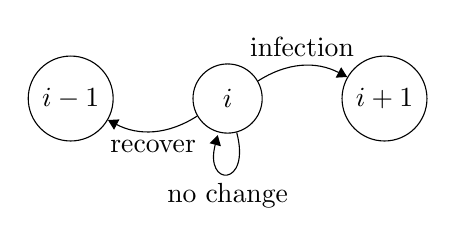
\begin{tikzpicture}[start chain = going right,
   -Triangle, every loop/.append style = {-Triangle}]
   \node[state, on chain]  (h) {$i-1$ };
   \node[state, on chain]  (i) {$i$ };        
   \node[state, on chain]  (j) {$i+1$ };

   \draw(i) edge[loop below, "no change"] (i);
   \draw(i) edge[bend left, "recover"] (h);
   \draw(i) edge[bend left, "infection"] (j);
\end{tikzpicture}
\end{document}